\chapter{Origins of Multi-decadal Variability in Sudden Stratospheric Warming events}
\label{cha:models}
\begin{quotation}
  Much of the work presented in this chapter is based on Dimdore-Miles et al. 2020 (ref) however the analysis has been extended here to include a more comprehensive diagnosis of stratospheric variability in the UKESM gcm.
\end{quotation}


\section{Introduction}
\label{sec:origins_introduction}
Despite a significant body of work aimed at understanding the nature of vortex variability including SSWs, variations in this mode on decadal to multi-decadal timescales is not well understood. A formal diagnosis of such variability as well as a better understanding of factors which influence it may help to improve predictability of SSWs and subsequently NH mid-latitude surface climate.

Nevertheless, some studies have addressed the notion of low frequency variations in the vortex. \cite{Garfinkel2017} analyse decadal-scale variations in vortex strength in a set of historical simulations and propose that an observed hiatus in Eurasian surface warming was most likely due to variability in midwinter vortex strength. Similarly, \cite{cohen2009} find decadal scale variations in planetary wave forcing of the vortex in a suite of CMIP3 models as well as NCEP–NCAR reanalysis. Whether the vortex variability was forced by greenhouse gas concentrations or arose through internal variability in these studies was not fully established but \cite{Garfinkel2015} used a subset of the simulations analysed in \cite{Garfinkel2017} and linked a decadal trend (1980-2009) in late winter vortex strength to SST variability. On the other hand, \cite{Seviour2017} analysed observed variations between 1980 and 2016 and concluded that the vortex variability was primarily internally generated. Other studies also point towards internally generated decadal fluctuations in vortex strength: \cite{Manzini2012} explore causes of 20 year period variability in a simulation with prescribed, pre-industrial SSTs. They propose that, given the boundary conditions in the simulations are fixed, such variability must be internally generated. Finally, \cite{Butchart2000} suggest that decadal variability in vortex strength as well as SSW frequency may originate from feedbacks caused by the non linear nature of boreal winter stratospheric dynamics.

On longer timescales, \cite{Schimanke2011} noted variations in SSW occurrence with periods of approximately 52 years in a multi-century GCM integration and demonstrated coherent variability in other parts of the climate system, including vertically propagating planetary wave activity, Eurasian snow cover and Atlantic SSTs. However, despite providing some indications of externally driven variability, results from this study are not conclusive, since the GCM used (EGMAM: ECHO‐G with Middle Atmosphere Model) exhibits significant bias in mean SSW rate compared to reanalyses (2 events per decade). The authors also note that further simulations are required to understand this variability. 

multi-decadal scale variations in climate features which can couple with the vortex has also been explored. There are clear decadal variations in the period and phase transition timing of the QBO \citep{Pascoe2005,Anstey2008,Yang2016}. These may be linked to variations in the degree of 'stalling' of the QBO phase descent, which can cause more or less persistent wind direction at a given level.  A number of studies have also noted the transient nature of the strength of the HT relationship \citep{Lu2008,Lu14,Anstey2008,OspEA10}. \cite{Lu2008,Lu14} note that the mid-latitude wave-guide is modulated by the shape of the vortex so that planetary waves are diverted further equatorwards when the vortex is anomalously strong and wide, and this could temporarily reduce the influence of the QBO on the vortex. The AL also varies significantly on decadal to multi-decadal timescales. \cite{Overland1999} note that 10 year mean values of SLP over the AL region exhibit fluctuations of up to 35\% of the climatological mean. Subsequent studies corroborate the presence of these decadal scale fluctuations: \cite{SUGIMOTO2009} and \cite{Minobe} show 20 year fluctuations in intensity and centre of action of the AL while \cite{Raible2005} propose a 50-60 year trend in AL intensity, suggesting the existence of even longer timescale variability. 

\section{Data And Methods}
\subsection{Model Configuration}
For analysis of multi-decadal variability in the vortex and SSWs, we utilise a simulation of the first version of the UK Earth System Model (henceforth referred to as UKESM), the most recent configuration of the MetOffice unified model (the UM) \citep{Mulcahy2018}. UKESM is a stratosphere resolving coupled ocean-atmosphere-land-sea ice model. The Atmospheric component is GA7.1 with 85 vertical levels from the surface to 85km, 35 of which are above 18km \citep{Walters2019, Williams2018}. The model is run at N96 horizontal resolution (approximately 135 km near the equator). The ocean model used is GO6.0 \citep{Storkey2018} which contains 75 levels and runs at 1${^\circ}$ horizontal resolution. Land surface and sea-ice processes are represented by JULES \citep[GL7.0,][]{Walters2019} and CICE  \cite[GSI8.1,][]{Ridley2018} models respectively, while ocean biochemistry is added through MEDUSA \citep{Yool2013}. UKESM also includes a fully interactive chemistry scheme via coupling with the UK Chemistry and Aerosols model \citep[UKCA,][]{Mulcahy2018}.

We utilise a 1000 year pre-industrial (PI) control simulation of UKESM submitted to CMIP6 which is spun-up to achieve initial model equilibrium following the method outlined in \cite{Yool20}. This run is forced using CMIP6 pre-industrial values for concentrations of major GHGs (global mean 284.317ppm $CO_2$, 808.25ppb $CH_4$, 273.02ppb $N_2O$). While there are no volcanic eruptions in the simulation, background stratospheric volcanic aerosols are set to climatological values between 1850 and 2014 estimated from satellite products and other model simulations \citep{Menary2018}. We choose a PI control for this analysis to examine internal variability in SSWs on multi-decadal timescales. 


\subsection{Reanalysis Data}
To verify that the model reproduces relevant features of the climate system we compare with an observation based dataset produced by the ECMWF - ERA-Interim \cite{Dee2011}. The ERA-interim dataset is produced by a 4D-Var data assimilation method of a wide range of observations \citep{Uppala2005}. These include surface measurements, aircraft campaign data, radiosonde readings and satellite observations. The 4D-var data assimilation process involves supplying the ECMWF’s Integrated Forecast System (IFS) initial conditions from observations, letting the model evolve for a timestep and re-initialising for the next step with a combination of output and updated observations \citep{Courtier1998, Bouttier2001}. This update is carried out to minimise a cost function defined to capture the difference between the latest model output and observations for that corresponding time. ERA-Interim provides data on 60 vertical levels at a maximum horizontal resolution of $\sim$ 80 km from 1979-2019 \citep{Berrisford}.

The majority of observations assimilated for ERA-Interim are satellite based radiance retrievals. These are gained from nadir facing satellites which measure spectral radiances (energy detected at difference wavelengths). A single detection device will consist of several channels which detect radiation from difference wavelengths. Different atmospheric layers absorb and emit at different wavelengths so measuring over a range of channels can build up a vertical profile of temperature (for example). However, the atmospheric layers that are detected by each channel may overlap resulting in measurements from multiple channels being used in the retrieval of a given layer. A weighting is applied to the channels at each height to account for the proportion of the total measurement that should be contributed by each channel. Channel weighting profiles (figure \ref{fig:Satellite_channels}) \citep{Fujiwara17} are generally Gaussian (for Nadir Satellites) in pressure, the width of which signifying the vertical extent of the channel. The vertical resolution of the retrievals is determined by the density of channels covering a particular height range. 

During the ERA-Interim period, the set of observations used for assimilation have developed significantly. Between 1979 and 1998 only limited satellite based radiance retrievals are available to produce profiles. These satellite observations are primarily provided by the Stratosphere Sounding Unit (SSU) and Microwave Sounding Unit (MSU) which are parts of the TRIOS Operational Vertical Sounder (TOVS) suite. The SSU possesses only 3 channels (figure \ref{fig:Satellite_channels}a) and therefore provides data at relatively coarse vertical resolution. Over this period, ERA-interim relies heavily on direct measurement techniques such as radiosondes, dropsondes and aircraft \citep{Fujiwara17} which bring possible biases from the influence of shortwave solar heating on temperature sensors in radiosondes as well as warmer tendencies in aircraft based observations compared to radiosondes \citep{Ballish2008}. After 1998 more extensive satellite based measurements are available for assimilation and are incorporated in ERA-interim. The new satellite products include improved versions of the SSU and MSU as a part of the Advanced TRIOS Operational Vertical Sounder (ATOVS) suite which provides profiles derived from the Advanced Microwave Sounding Unit A (AMSU, figure \ref{fig:Satellite_channels}b) from which ERA-interim calculates profiles using 11 channels (channels 5-14 from AMSU). ERA-Interim also makes use of a number of other satellite based instruments which are fully outlined in \citep{Fujiwara17}. Possible sources of biases in these satellite based observations include orbital drift and calibration offsets \citep{Zou2006,Simmons2014}.

As a result of including additional observations for assimilation after 1998, ERA-interim shows a shift in temperature structure of the middle and upper stratosphere between the two periods. Caution is therefore, advised when using this data for trend analysis \citep{Long2017} however such an analysis does not form part of the work in this thesis. Zonal wind fields show little change across the periods. Additionally, ERA-interim struggles (as the majority of modern reanalyses do) to constrain phase transition timing of the QBO correctly \citep{Kawatani2016}. Comparisons with wind profiles derived from a single radiosonde station, Singapore at $^{\circ}$1N, $104^{\circ}$E, which covers a large majority of the reanalysis period, show that ERA-interim also exhibits biases in the amplitude of both QBO phases. These biases reduce significantly with the transition to the use of ATOVS \citep{Kawatani2016,Long2017}. Similar biases and improvements over the TOVS-ATOVS period are also observed for representation of the SAO \cite{BaldwinGray2005}. These biases must be taken into account when considering comparisons in stratospheric circulation between ERA-interim and GCMs. Nonetheless, \cite{Long2017} stress that these datasets are in broad agreement with other major reanalyses in the stratosphere and lower mesosphere.

\begin{figure}[h!]
\centering
    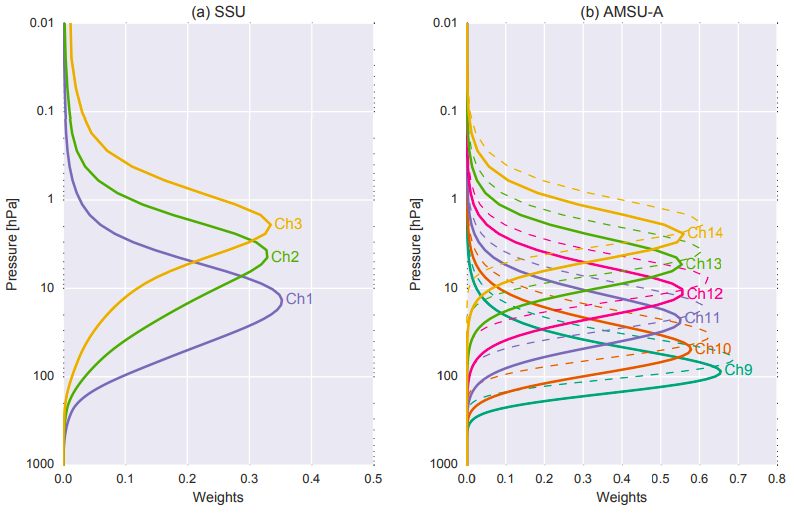
\includegraphics[width=0.5\textwidth]{Figures/Figures-origins/channels.png}
    \caption[Channel profiles for satellite retrievals assimilated by ERA-Interim]{Figure from \cite{Fujiwara17} \textbf{Left}: Channel weighting profiles for the TOVS Stratospheric Sounding Unit (SSU) used for ERA-Interim dataset in the period 1979-2005. \textbf{Right}: Weighting profiles from the ATOVS-suite Advanced Microwave Sounding Unit (AMSU) which provides measurements for ERA-Interim from 1998-present. Solid lines represent near Nadir profiles and dashed lines signify limb profiles (taken at an angle of $48.33^{\circ}$).}
    \label{fig:Satellite_channels}
\centering
\end{figure}

\subsection{Wavelet Analysis}
\label{sec:Wavelet_Analysis}
In order to study possible multi-decadal variability in SSW occurrence, we utilise a wavelet analysis method based on \cite{Torrence1998}. Such an analysis can be used to examine time series which displays non-stationary spectral power over multiple frequencies \citep{Daubechies} giving it a useful advantage over more traditional fourier methods for spectral analysis. The wavelet transform of a uniform 1-dimensional time series, $x$, of length $N$ and timestep $\delta t$ is given by the convolution between the series and a scaled and translated version of a wavelet function $\psi_0$ (equation \ref{wavelet_transform})

\begin{equation} \label{wavelet_transform}
W_n(s) = \sum^{N - 1}_{n' = 0} x_{n'} \psi^* \bigg[(n' - n) \frac{\delta t}{s}\bigg],
\end{equation}

where $*$ denotes the complex conjugate and $s$ is the wavelet scale indicating the frequency of the wavelet. Varying $s$ and translating along the time scale (the index $n$), $W_n$ indicates the amplitude of signals at different scales and their variation in time. \cite{Torrence1998} suggest an approach to varying the scale s as increasing in powers of 2 according to 

\begin{equation} \label{S}
s_j = s_0 2^{j \delta j},\\ j = 0, 1, ..., J
\end{equation}

\begin{equation} \label{S}
J = \delta j^{-1} log_2\bigg(\frac{N \delta t}{s_0}\bigg),
\end{equation}

where $s_0$ is the shortest resolvable scale of a signal, J corresponds to the longest and $\delta j$ is the scale resolution. The translated and scaled wavelet has the form

\begin{equation} \label{wavelet}
\psi^* \bigg[(n' - n) \frac{\delta t}{s}\bigg] = \bigg(\frac{\delta t}{s}\bigg)^{1/2} \psi_0\bigg[(n' - n) \frac{\delta t}{s}\bigg]
\end{equation}

and we select the form of $\psi_0$ following the recommendation of \cite{Torrence1998} as a Morlet wavelet, an oscillatory function enveloped by a Gaussian which is expressed as

\begin{equation} \label{psi0}
\psi_0(p) = \pi^{-1/4} e^{i\omega_0 p} e^{\frac{p^2}{2}}.
\end{equation}

The advantages of using a Morlet wavelet for analysing signals in climate time-series is discussed in \cite{Lau1995} in which the authors acknowledge that while truly physical signals should be detected regardless of which wavelet basis is chosen, for best results one should adopt a wavelet function reminiscent of the real signal. They show that when a Morlet wavelet form is utilised, spectral decomposition methods can detect common forms of behaviour exhibited in the variability of time series associated with the Earth's climate. These include time variations in period and amplitude of signals, abrupt changes in periodicity (sudden regime shift to different spectral behaviour) and some forms of rapid changes in series over time. These forms of behaviour are most likely relevant for our analysis of SSWs, therefore we proceed with a wavelet of this form. 

It is computationally quicker to compute the wavelet transform in discrete Fourier space. By the convolution theorem, the transform reduces to multiplication

\begin{equation} \label{wavelet_transform2}
W_n(s) = \sum^{N - 1}_{k = 0} \hat{x}_{k} \hat{\psi}^* (s\omega_k) e^{i \omega_k n \delta t},
\end{equation}

where $\hat{x}_{k}$ and $\hat{\psi}$ are the discrete Fourier transforms of the time series $x$ (equation \ref{fourier1}) and the wavelet function (equation \ref{fourier2}) respectively,

\begin{equation} \label{fourier1}
\hat{x}_k = \frac{1}{N} \sum^{N-1}_{n = 0} x_n e^{\frac{-2\pi i k n}{N}}
\end{equation}

\begin{equation} \label{fourier2}
\hat{\psi}(s\omega_k) = \bigg(\frac{2 \pi s}{\delta t}\bigg) \pi^{-1/4}H(\omega_k) e^{-(s\omega_k - \omega_0)^2/2}.
\end{equation}

$H(\omega_k)$ is the Heavyside function and $\hat{\psi}$ is normalised to have unit energy when integrated over all $\omega$. The square modulus of the wavelet transform gives the wavelet power spectrum which indicates relative strength of signals in the time series as a function of signal period and discretised time. In order to directly compare spectra of different indices we normalise all spectra by the variance of the corresponding time series. We also define a confidence interval for wavelet power observed at a given period and time for a series by assuming a mean background spectrum corresponding to that of a first order autoregressive (AR1, red noise) process modelled by

\begin{equation} \label{rednoise}
x_n = \alpha x_{n - 1} + z_n,
\end{equation}

where $\alpha$ is the lag-1 autocorrelation of the time series and $z_n$ is Gaussian white noise. \cite{Torrence1998} show that such a process's wavelet power spectrum is $\chi^2$ distributed and therefore can be used to define a 95\% confidence interval for any observed power. 

\subsubesection*{Cross Wavelet Spectra}
The cross wavelet spectrum of two time series $x$ and $y$ with associated wavelet spectra $W^x_n$ and $W^y_n$ gives a measure of coincident power (the same period at the same timepoints) between the series. It is given by

\begin{equation} \label{wavelet_cross}
\vert W^{xy}_n(s)\vert = \vert W^{x*}_n(s) W^{y}_n(s)\vert,
\end{equation}

where $W^{x*}_n(s)$ is the complex conjugate of the wavelet power spectrum of $x$ \citep{Grinstead2004}. The complex argument of $W^{xy}_n(s)$ gives the local phase difference between signals in $x$ and $y$ in frequency-time space. The phase relationship between the two time-series can be represented by a
vector that subtends an angle representing the phase difference: On all plots of cross spectra, arrows to the right (left) denoted signals which are in-phase and correlated (anti-correlated). Vertical arrows indicate a phase relationship of $\frac{\pi}{2}$ between the time-series, so that the evolution of
one is correlated with the rate-of-change of the other. As for individual power spectra, we define a confidence interval for which cross power of a larger amplitude is deemed significant (>95\% confidence interval) by comparing power exhibited by actual series with a theoretical red noise process. The cross power of two such AR1 processes is theoretically distributed such that the probability of obtaining cross power greater than a set of red-noise processes is

\begin{equation} \label{wavelet_cross_dist}
D\bigg(\frac{\vert W^{xy}_n(s)\vert}{\sigma_x \sigma_y} < p\bigg) = \frac{Z_\nu(p)}{\nu} \sqrt{P^x_k P^y_k},
\end{equation}

where $\sigma$ denotes the standard deviation of the time series, Z is the confidence interval defined by $p$ ($Z$ = 3.999 for 95\% confidence), $\nu$ is the degrees of freedom for a real wavelet spectrum ($\nu$ = 2) and $P^x_k$ is the theoretical Fourier spectrum of the AR1 process. For a given wavenumber k, this can be expressed as

\begin{equation} \label{theoretical_fourier}
P_k = \frac{1 - \alpha^2}{\vert 1 - \alpha e^{2i\pi k} \vert^2}.
\end{equation}

\subsection{Hilbert Transform}
We utilise a signal processing method known as a Hilbert transform to calculate the instantaneous phasor amplitude of a QBO time series. The Hilbert transform of a time series $x(t)$ can be expressed as

\begin{equation} \label{theoretical_fourier}
\tilde{x} = Hil[x(t)] = \frac{1}{\pi t} * x(t),
\end{equation}

where $\tilde{}$ denotes the transformed series, * signifies a convolution and $t$ is discretised time. Conversely, the original time series can be recovered using an inverse transform expressed as

\begin{equation} \label{theoretical_fourier}
{x(t)} = Hil^{-1}[\tilde{x}(t)] = -\frac{1}{\pi t} * \tilde{x}(t).
\end{equation}

A complex signal which consists of $x(t)$ and its transform is known as the analytic signal of $x$ and can be used to calculate an instantaneous phasor amplitude, $A(t)$, of the signal. $X(t)$ can be expressed as

\begin{equation} \label{theoretical_fourier}
X(t) = x(t) + \tilde{x}(t) i = A(t) e^{i\theta},
\end{equation}

where $A(t)$ is the instantaneous amplitude of the signal and $\theta(t)$ is the instantaneous phase angle - a measure of signal progression through a cycle at time $t$.

\subsection{Statistical Methods}
\label{sec:stat_tests}

\subsubsection*{Student's t-test}
Much of the analysis presented in this chapter, and indeed in the whole thesis, involves comparisons of composite and mean quantities. A two-tailed student's t-test is implemented to test the null hypothesis that two sampled quantities, $x_1$ and $x_2$, with means $\overline{x}_1$ and $\overline{x}_2$ and standard deviations $\sigma_{1}$ and $\sigma_{2}$ are drawn from the same underlying normal distribution. A $t$ statistic is defined by $t = \frac{\overline{x}_1 - \overline{x}_2}{\sigma_{12} \sqrt{\frac{1}{n_1} + \frac{1}{n_2}}}$ where $n_i$ is the number of samples for quantity $i$ and $\sigma_{12}$ is the pooled variance for the two quantities given by $\sigma_{12} = \sqrt{\frac{\sigma^2_2 (n_2-1) + \sigma^2_1(n_1 - 1)}{n_1+n_2-2}}$. Significance on the difference in means can then be estimated by comparing the value of $t$ with a Student's t-distribution to give an associated $p$ value. Differences which give a $p$ value greater than a deemed level (normally 95\%) are deemed significant in which case the null hypothesis of identical means is rejected to this level.

\subsubsection*{Linear Regression Analysis}
We employ a multi-linear regression technique to give an estimate of the relative contributions to SSW variability from the QBO, ENSO and the AL following the method outlined in \cite{Krzywinski}. We model an SSW timeseries of length $n$ which we denote $y$ as 

\begin{equation} \label{regression}
\hat{y} = \beta_0 + \beta_{1}QBO + \beta_{2}ENSO + \beta_{3}AL
\end{equation}

where $\beta_j$ denotes the coefficient of the corresponding index and $\hat{y}$ is the prediction of $y$. We calculate the best estimate for each $\beta$ using an ordinary least square (OLS) estimator which minimises the sum of squared error (SSE) between the predicted $\hat{y}$ and the real time series $y$ with respect to each coefficient. the SSE is given by $SSE = \sum_i^n{(\hat{y}_i - y_i)^2}$.

We can compare the estimated magnitude of the coefficient for each index to analyse the respective contributions to SSW variability. We can also calculate standard error ranges for $\beta$ estimates. The standard error on an estimated value of a true $\beta_j$ (denoted by $\hat{\beta_j}$) is given by 

\begin{equation} \label{regression}
se(\hat{\beta_j}) = \sqrt{\frac{SSR}{n - k} (X^TX)^{-1}_{jj}}
\end{equation}

where SSR is the sum of squared residuals which measures the sum of squared deviations of predicted values from the mean $y$ value, $\overline{y}$. This is given by $SSR = \sum_i^n{(\hat{y}_i - \overline{y})^2}$). $k$ is the number of predictors used in the linear model (in this case 3) and $X$ is an $n \times k$ matrix consisting of the predictor indices. We also define significance levels for $\hat{\beta_j}$ using a one-tailed $t$ statistic (similar to above) with $n-k$ degrees of freedom to test the null hypothesis that $\hat{\beta_j}$ = 0. The $t$ statistic is given by $t = \frac{\hat{\beta_j}}{se(\hat{\beta_j})}$.

\subsubsection*{SSW Statistics}
In order to assess model representation of vortex variability, we introduce a statistical framework which uses parametric and bootstrapping methods to asses significance levels for differences in SSW abundance across datasets. First, a parametric approach which assumes that the occurrence of any number of SSWs (denoted as $N$) in a given number of winters (denoted by $k$) can be modeled as a Poisson process and is distributed as 

\begin{equation} \label{Poisson}
P(N(k) = n) = \frac{(\lambda k)^n}{n!} e^{-\lambda k},
\end{equation}

where $\lambda$ is the intensity of the Poisson process calculated as the mean SSW rate over $k$ winters. For two such processes with intensities $\lambda_1$ and $\lambda_2$ the difference in intensity, $\Delta\lambda$ can be expressed as

\begin{equation} \label{Poisson}
\Delta\lambda = \frac{\lambda_1 - \lambda_2}{\sqrt{\frac{\lambda_1}{k_1} + \frac{\lambda2}{k_2}}},
\end{equation}

where $k_i$ is the number of instances of process $i$ (number of winters sampled). \cite{Charlton2007} suggest that if a pair of Poisson processes are recorded for more than 30 instances each then $\Delta\lambda$ can be assumed to be normally distributed. \cite{Gu} and \cite{Huffman} present an alternative test for the significance of $\Delta\lambda$ in cases where the datasets underlying each process are of different lengths (i.e. for comparing model and reanalysis data). For this analysis, we introduce the test statistic

\begin{equation} \label{deltalambda}
W(X_1, X_2) = 2 \frac{\sqrt{X_1 + 3/8} - \sqrt{\rho(X_2 - 3/8)}}
{\sqrt{1 + \rho}},
\end{equation}

where $\rho$ is the ratio of observation lengths of the datasets and $X_i$ is the number of observations of events (number of SSWs) in dataset $i$. W is distributed with associated an $p$ value, 

\begin{equation} \label{Pval}
p = 1-2\psi(W(X_1, X_2)),
\end{equation}

where $\psi(W)$ is the cumulative distribution function of the normal distribution. This statistic provides a parametric test for significance between different SSW rates and the associated p-value is referred to as $P_{para}$ to distinguish it from other tests. 

Additionally, we utilise a bootstrapping approach to test significance in SSW rate differences. For this method we assume two datasets produce a set of time series of the number of SSWs in each winter. These are denoted as $[X1,X2.....X_k]$ and $[Y1,Y2.....Y_j]$ and the mean SSW rate can be expressed as $\mu_X = \frac{\sum[X_1,X_2.....X_k]}{k}$. A confidence interval for an observed difference in mean SSW rate ($\Delta\mu = \mu_X - \mu_Y$) can be constructed by forming a pooled dataset, $Z = [X_1, X_2,....X_k,Y_1,Y_2,....Y_j]$ and randomly choosing (without replacement) synthetic datasets of the same length as $X$ and $Y$ from $Z$ and subsequently calculating synthetic mean differences. repeated choosing can build up a distribution for mean differences and a confidence interval for the real difference, $\Delta\mu$. We perform a set of 10000 random choices for this statistical test and the associated $p$ value is referred to as $P_{boot}$.


\subsection{Model Diagnostics}
We utilise the definition of an SSW event from \cite{Butler2015}. An event is recorded when the ZMZW at 60$^\circ$N on the 10\,hPa level transitions from westerly to easterly during NH winter months (November - March). The day on which this reversal occurs is referred to as the central date. After this date, the ZMZW must recover to westerly for a period of at least 10 consecutive days (which is the approximate radiative timescale of the mid-stratosphere) before another event can be recorded.  If, after the central date, the ZMZW does not recover to westerly for at least 20 consecutive days before the end of April, the warming is classified as a final warming. While we do record all events in extended winter (Nov-Mar) for an initial analysis of mean SSW rates, we use mid-late winter warmings (Dec-Mar) for our analysis of multi-decadal variability and interaction with other other climate variables (this choice is addressed in section \ref{sec:strat_var_UKESM}). We also use the NAM as a continuous metric for vortex strength following the methodology of \cite{baldwinStratospheric2001}. the $NAM_{10}$ index is defined as the leading Principle Component of the deseasonalised GPH field evaluated over the winter months (Dec-Mar, as with SSWs) on the 10hPa level. Utilising this metric gives the advantage of encoding both anomalously weak vortex winters (which include SSWs) as well as those in which the vortex is anomalously strong. In contrast, the use of the use of the ZMZW definition of an SSW gives a discretised metric of weak events (or absence of them) which may influence its spectral characteristics. This discretisation compared to the NAM definition is discussed in section xxxx.

We analyse variability in tropical SSTs in four regions identified by \cite{Scaife2016} as key to affecting Rossby wave propagation and interactions with stratospheric winds. The regions are defined as the Tropical Atlantic ($5^{\circ}S$-$5^{\circ}N, 60^{\circ}W$–$0^{\circ}W$), Tropical East Pacific ($5^{\circ}S$–$10^{\circ}N, 160^{\circ}$–$270^{\circ}E$), Tropical West Pacific ($5^{\circ}S$–$25^{\circ}N, 110^{\circ}$–$140^{\circ}E$) and Tropical Indian Ocean ($5^{\circ}S$–$10^{\circ}N, 45^{\circ}$–$100^{\circ}E$). Additionally we calculate an El Ni\~{n}o Southern Oscillation (ENSO3.4) index as the SST anomaly in the region $5^{\circ}S$-$5^{\circ}N, 170^{\circ}W$–$120^{\circ}W$ following \cite{Trenberth2001}. We use an index to track the intensity of the Aleutian low pressure system based on the method of \cite{Chen2020} as the projection of the first Principal Component of winter mean sea level pressure (MSLP) anomalies averaged over the region $120^{\circ}$–$240^{\circ}E, 20^{\circ}$–$70^{\circ}N$. We employ an EOF based method as opposed to a fixed box average to allow for the fact that the centre of the model AL may not line up well with observations. The month range used for studies into AL-vortex teleconnections varies somewhat with \cite{Overland1999} using both Jan-Feb and Nov-Mar while \cite{Hu2018} use a core winter metric (Dec-Feb). Unless stated otherwise we use the same month range as our SSW definition (Dec-Mar); for all analyses, tests were performed to check that the results were not unduly sensitive to the choice. An index for the Pacific Decadal Oscillation (PDO) was determined following the methodology of \cite{Mantua_1997} using the leading Principal Component of Pacific basin ($120^{\circ}$–$240^{\circ}E$) SST anomalies poleward of 20$^{\circ}$N. Finally, a QBO index was defined by a variety of measures (see section 3 for further discussion), using the monthly mean ZMZW averaged between $\pm5^{\circ}$ latitudes at various stratospheric pressure levels (15\,hPa, 20\,hPa, 30\,hPa, 50\,hPa, 70\,hPa) as well as two 'deep QBO' indices computed  by taking the average of the ZMZW between  15-30\,hPa (as in \cite{andre}) and between 20-50\,hPa to identify QBO phases that exhibit winds of the same sign over a relatively large vertical extent. 

\section{Results}
\subsection{Modes of Stratospheric Variability}
\label{sec:strat_var_UKESM}
We begin by analysing the representation of modes of stratospheric variability in the UKESM piControl simulation. As described in section 1, the winter polar stratospheric vortex  exhibits substantial variability. In some years the westerly winds of the vortex are relatively strong and undisturbed while in other years the vortex is weakened by wave disturbances that in extreme cases can lead to SSWs. The average Nov-Mar SSW rate over the full 1000 years of the UKESM simulation is 0.54 events/winter. This represents a marginal underestimation compared to ERA-Interim (0.62 events/winter between 1979 and 2019) but is within 1 standard error of the observations. The model adequately represents the seasonal distribution of SSWs compared to the reanalysis dataset, as shown in figure 1, but exhibits too many warming events in November (not shown) and an underestimation of Jan and Feb warming rates (see \cite{Andrews2020} and \cite{Menary2018} for further details). This bias is well known and relatively common in GCMs \citep{Charlton2007, Ayarz2020}. On the other hand, we note that validation of this pre-industrial control simulation with ERA-Interim data is not optimum. The sample sizes of the ERA-interim data and the model are very different and could give rise to differences in distributions \citep{Horan2017} and the ERA-Interim SSW rates may be influenced by anthropogenic forcing, the impact of which is not well understood \citep{Ayarz2020}. In all analyses presented in the following sections, tests have been performed to ensure that the results are not sensitive to the inclusion or exclusion of November SSW rates. 

\begin{center}
\begin{figure}[h!]
\noindent\includegraphics[width = 0.5\linewidth]{f01.png}
\caption{SSWs per NH winter season separated by month within the UKESM pi-control and ERA-Interim datasets. Error bars are derived using a bootstrap re-sampling method in which random selections of 50 years are chosen from the SSW data and the SSW rate recorded to build a PDF of events per season. 10000 such re-samples are carried out and the 97.5 and 2.5 percentile values are used as error bounds.}
\label{fig1}
\end{figure}
\end{center}

The model exhibits variability in SSW frequency comparable to observations, including both hiatus and consecutive SSW intervals. Figure 2 shows a sample 40-yr interval of the polar vortex zonal wind strength from the UKESM simulation compared with a similar length from the ERA Interim reanalyses. An extended interval of mainly westerly anomalies indicating a strengthened vortex and lack of SSWs can be seen towards the end of the 40-yr interval, similar to the 1990s in ERA-Interim when only 2 SSW events were recorded in the decade. The simulation contains 8 such hiatus intervals with at least 10 consecutive years with no SSWs, the longest of which lasts 16 years. On the other hand, the simulation only contains 2 intervals in which 10 consecutive years exhibit at least 1 SSW. However, if the threshold interval width for identifying hiatus and consecutive-SSW intervals is shortened from 10 to 5 years,  then 9 consecutive-SSW intervals and 25 hiatus intervals are found. These statistics indicate that UKESM is not only able to reproduce the mean state characteristics of SSW events but also decadal-scale variations in SSW rate, underlining its  suitability for this study. 

The second major mode of stratospheric variability is the QBO at equatorial latitudes which is present at all times of the year. Figure 3 shows the equatorial wind time-series from a sample 40-yr interval of the simulation compared with the ERA-Interim dataset. The mean period of the oscillation is longer than observed, at $\sim$38 months compared to $\sim$28 months in ERA-Interim \citep{Kawatani2016}. As a result the vertical shear zones descend less rapidly than observed. There is also a westerly bias at low levels where the QBO-E phase does not extend sufficiently deep into the lower stratosphere, which is a common bias in many models \citep{Bushell2020}. The descending shear zones also appear more regular than observed but there is nevertheless some evidence of decadal-scale variations e.g. in the degree of stalling at 30\ hPa, although not as pronounced as in the observations.

\begin{center}
\begin{figure}[h!]
\noindent\includegraphics[width = \linewidth]{f02.png}
\caption{\textbf{(a, b)}: Dec-Mar annual mean ZMZW anomaly from the climatological mean at 60$^\circ$\,N from a 40 year sample from the pre-industrial control simulation of UKESM \textbf{(a)} and the ERA-Interim dataset between 1979 and 2018 \textbf{(b)}. \textbf{(c, d)}: Time series of SSWs recorded per winter season in the same datasets.}
\label{fig1}
\end{figure}
\end{center}

%---------------------------------------------------------------

\begin{center}
\begin{figure}[h!]
\noindent\includegraphics[width = 0.8\linewidth]{f03.png}
\caption{ZMZW averaged between 5$^{\circ}$\,S--5$^{\circ}$\,N latitude from from a 40 year sample of the pre-industrial control simulation of UKESM \textbf{(a)} and the ERA-Interim dataset between 1979 and 2018 \textbf{(b)} Horizontal lines mark the 15\,hPa and 30\,hPa levels between which the deep QBO metric employed by \cite{Andrews2019} is defined.}
\label{fig1}
\end{figure}
\end{center}


%---------------------------------------------------------------

There is evidence of coupling between the two major modes of stratospheric variability in the model, giving rise to a Holton-Tan relationship \citep{Anstey20}. Figure 4 shows height-latitude cross-sections of NH winter zonal wind differences between QBO E-W composites defined at various equatorial levels. The familiar pancake structure of alternating easterly / westerly differences is present at equatorial latitudes, indicative of the QBO phase but there is also a response at high latitudes. In good agreement with observations the largest high latitude response amplitude is seen when  the QBO is defined at 50hPa, with anomalously weaker polar vortex strength in QBO-E than in QBO-W years. Higher levels (15\,hPa and 20\,hPa) show little significant QBO-vortex coupling. For comparison we also show in figure 4 the composite different response for QBO composites selected on the basis of the average QBO winds over a greater depth of the equatorial atmosphere (15-30 hPa and 20-50 hPa). We note that while this QBO definition will select some of the same years as in the separate single-level composite definitions, it is specifically designed to identify only QBO  phases that have extended vertical coherence, following \citep{Gray2018} and \cite{Andrews2019}, so the resulting composite  differences in figure 4 will not necessarily be an average of the corresponding single-level differences.   Interestingly, the 15--30 hPa deep-QBO selects years that exhibit not only a weaker polar vortex in QBO-E but also a weaker sub-tropical tropospheric jet (see 200 hPa, 30--40N). This results in a more coherent response in the mid-latitude troposphere and at the surface, in excellent agreement with the results of \cite{Gray2018} and \cite{Andrews2019}. 

%---------------------------------------------------------------

\begin{center}
\begin{figure}[h!]
\noindent\includegraphics[width = 0.85\linewidth]{f04.png}
\caption{Dec-Mar ZMZW composite differences between QBO East and QBO West phases evaluated in Sep-Oct at individual levels as well as using the deep QBO metric. The phase of the QBO is defined as in figure 1 - the equatorial Sep-Nov ZMZW of greater magnitude than 5\ m\,s$^{-1}$. Coloured shading indicates differences significant above the 95\% confidence level under a 2 tail student’s t-test.}
\label{fig1}
\end{figure}
\end{center}

The presence of the Holton-Tan relationship is also seen in the modelled frequency of SSWs (figures 5). Significantly higher rates are observed in QBO-E winters than QBO-W. Also notable is the asymmetry in abundance of QBO-E and QBO-W winters - nearly twice as many QBO-E winters are observed compared to QBO-W under all phase definitions (figure 5, legends). This suggests an element of phase locking between the QBO and the seasonal cycle possibly associated with seasonally variations in the strength of mean equatorial upwelling or mid-latitude planetary wave forcing in winter \citep{Pascoe2005, Gruzdez2000, Kylash2015} resulting in QBO phase transitions that occur preferentially in certain months. 

\begin{center}
\begin{figure}[h!]
\noindent\includegraphics[width = 0.7\linewidth]{f05.png}
\caption{SSWs per winter season for years exhibiting QBO-E and QBO-W conditions in early winter (Sep-Nov) defined on different pressure levels (a,b) as well as using the deep metric (c), the vertical mean between 15 and 30\,hPa defined in \cite{Andrews2019}. The QBO phase is defined as any Sep-Nov equatorial ($5^{\circ}$\ S--$5^{\circ}\ $N average) ZMZW that exceeds a magnitude of 5\ m\,s$^{-1}$. Error bars on all plots are derived using the same bootstrapping method outlined in figure 1.}
\label{fig1}
\end{figure}
\end{center}





\subsection{Vortex-QBO Interactions}
Despite some coincident signals between tropical SSTs, AL and $SSW_{5yr}$, long-term variability in these surface indices are unable to fully account for the  multidecadal signals in SSW frequency. An additional potential source of internally generated long-term variability may reside within the stratosphere. Studies have noted relatively long-term variations in the strength of the Holton-Tan relationship \citep{Lu2008, Lu14, OspEA10} although the cause of these variations is not well understood. In order to investigate this figure 10 shows the wavelet power spectrum of early winter (Sep-Nov) QBO winds evaluated at selected levels. Since the QBO evolves relatively slowly, employing Sep-Nov averaged winds provides a reasonable representation of the QBO and also allows us to evaluate the in-season lagged relationship between the QBO and subsequent occurrence of an SSW. There is a clear signal between 2 and 4 years for the majority of the simulation, as expected, but no prominent power at longer periods,  confirming that there is no significant long-term variability in the periodicity of the QBO winds that could explain the long-term variations in $SSW_{5yr}$ via the Holton-Tan relationship.

\begin{center}
\begin{figure}[h!]
\noindent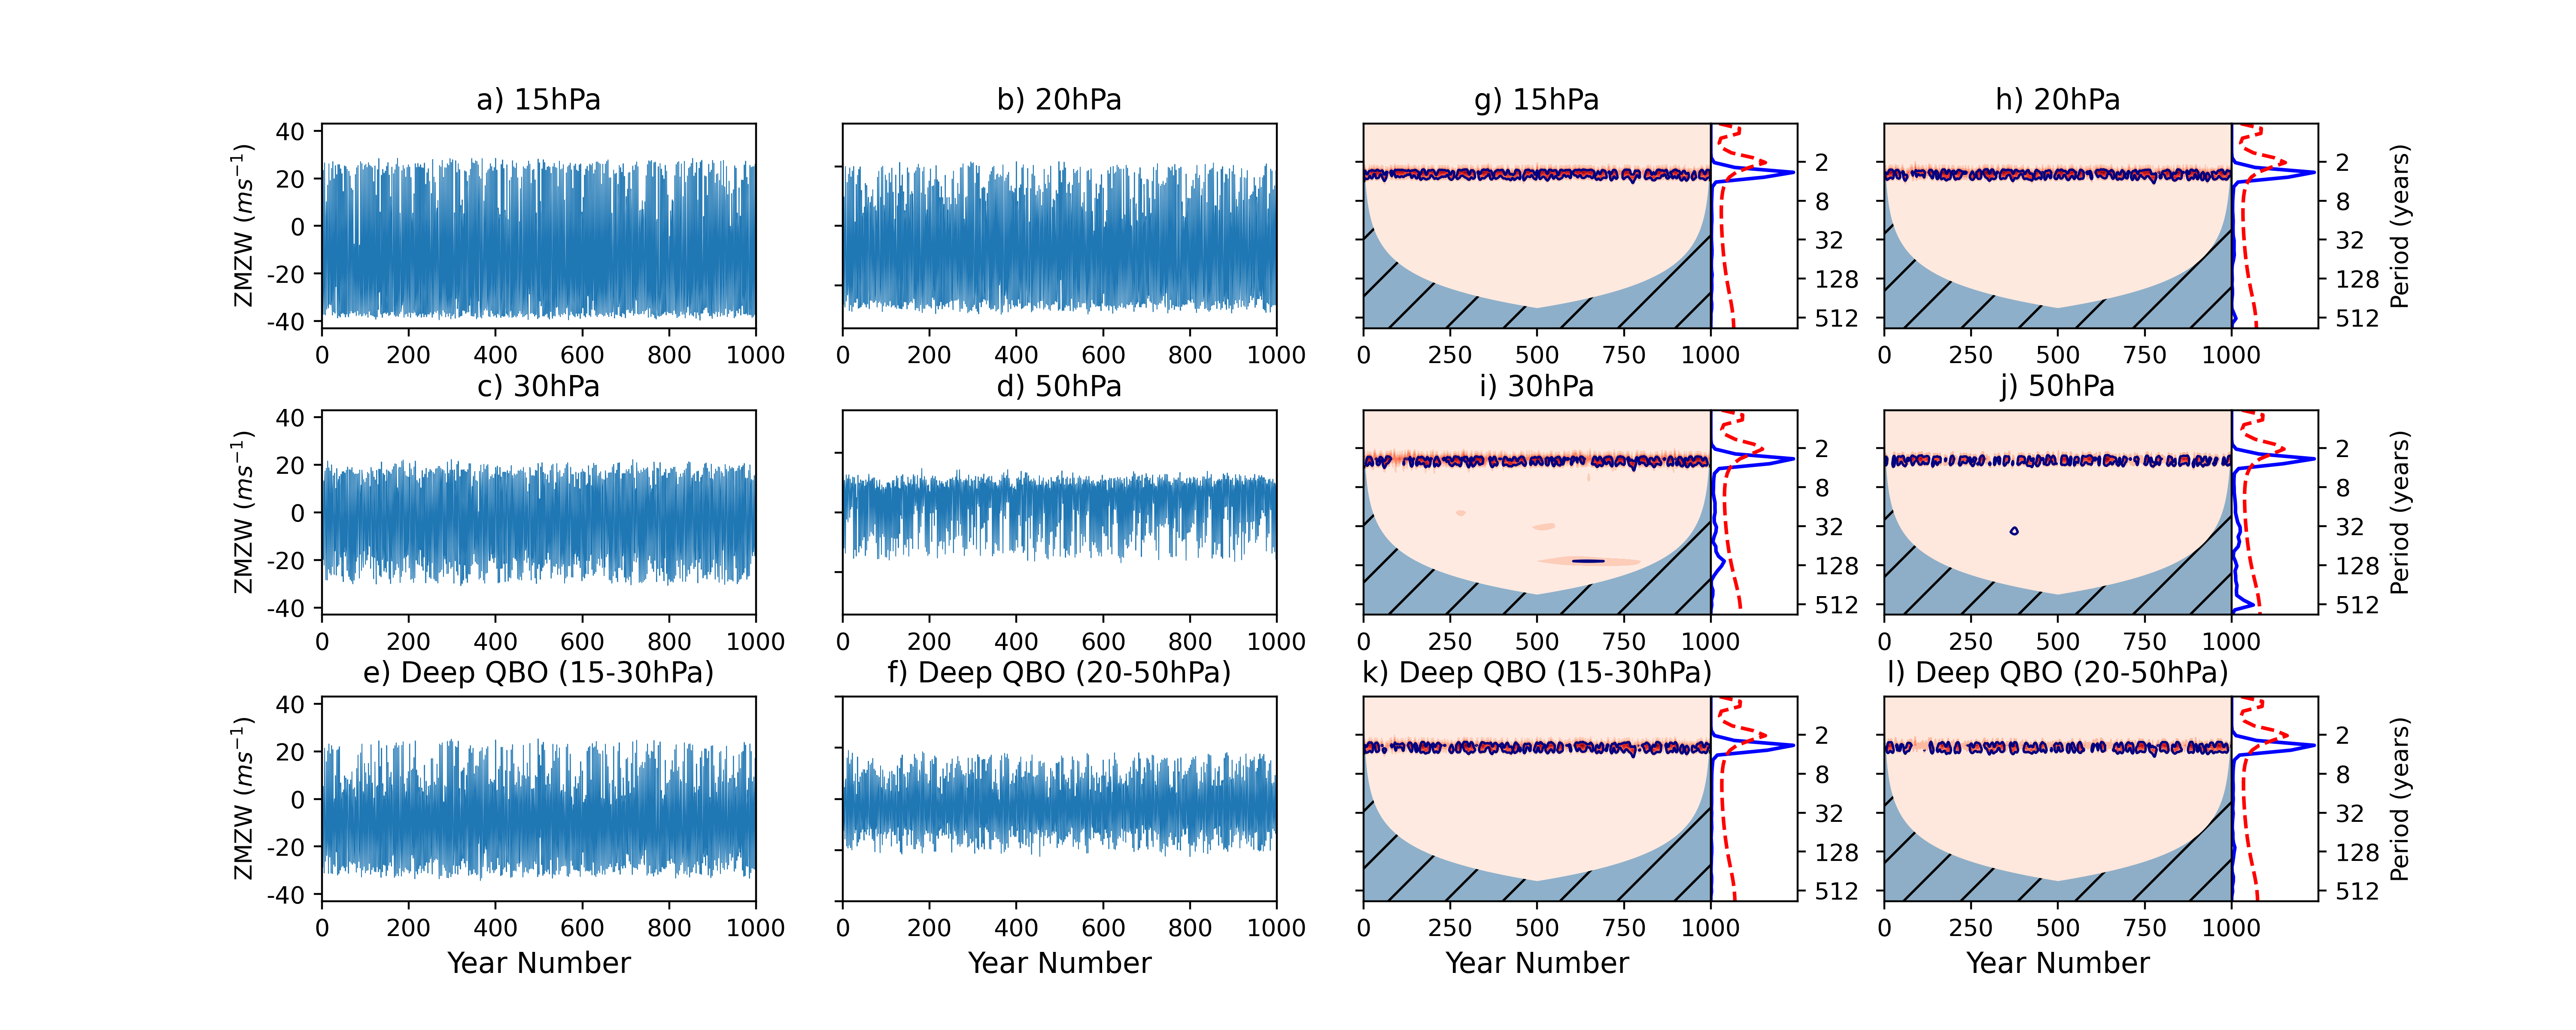
\includegraphics[width = \linewidth]{Figures/Figures-origins/QBO_levels.png}
\caption{\textbf{(a-f)}: Sep-Nov mean ZMZW averaged between 5$^\circ$S--5$^\circ$N latitude on different pressure levels (a-e) and the deep metric averaged between 15--30\,hPa (f). \textbf{(g-l)}: Wavelet power spectra for each time series shown in (a-c). Shading represents wavelet power with a colour scale the same as that seen in figure 6 and yellow contours indicate regions of significant power (>95\% confidence interval) compared to a background AR1 process.}
\label{QBO_levs}
\end{figure}
\end{center}

%---------------------------------------------------------------

While the wavelet analysis technique is able to isolate and reveal frequency modulations very well it is less suited to examine amplitude modulations which are clearly evident by eye in some of the QBO index time-series. For example, both the 20 hPa and deep (15-30 hPa) QBO time series show multi-decadal variations in the magnitude of the westerly phase while the easterly phase amplitudes are relatively uniform in time. Similarly, the 50\,hPa and 30\,hPa time series show amplitude modulation predominantly in the easterly phase. This amplitude modulation can be highlighted by taking the Hilbert Transform of each QBO time-series (figure 11a-f). Wavelet analysis of the transformed QBO time series now shows significant power on multidecadal timescales (figure 11g-l). In particular, the 20\,hPa and deep QBO time-series exhibit signals coincident in time and around similar periods (60-90 years) to those observed in $SSW_5yr$. On the other hand, the QBO indices based on equatorial winds at 50\,hPa or 30\,hPa show minimal power at these periods, despite showing a strong intraseasonal HT relationship (figure 4). Given that the 15-30 hPa deep QBO  index exhibits  both multidecadal timescale variability and a strong intraseasonal HT coupling, we continue further analysis of the SSW-QBO interactions using the 15-30 hPa index. 

%---------------------------------------------------------------

\begin{center}
\begin{figure}[h!]
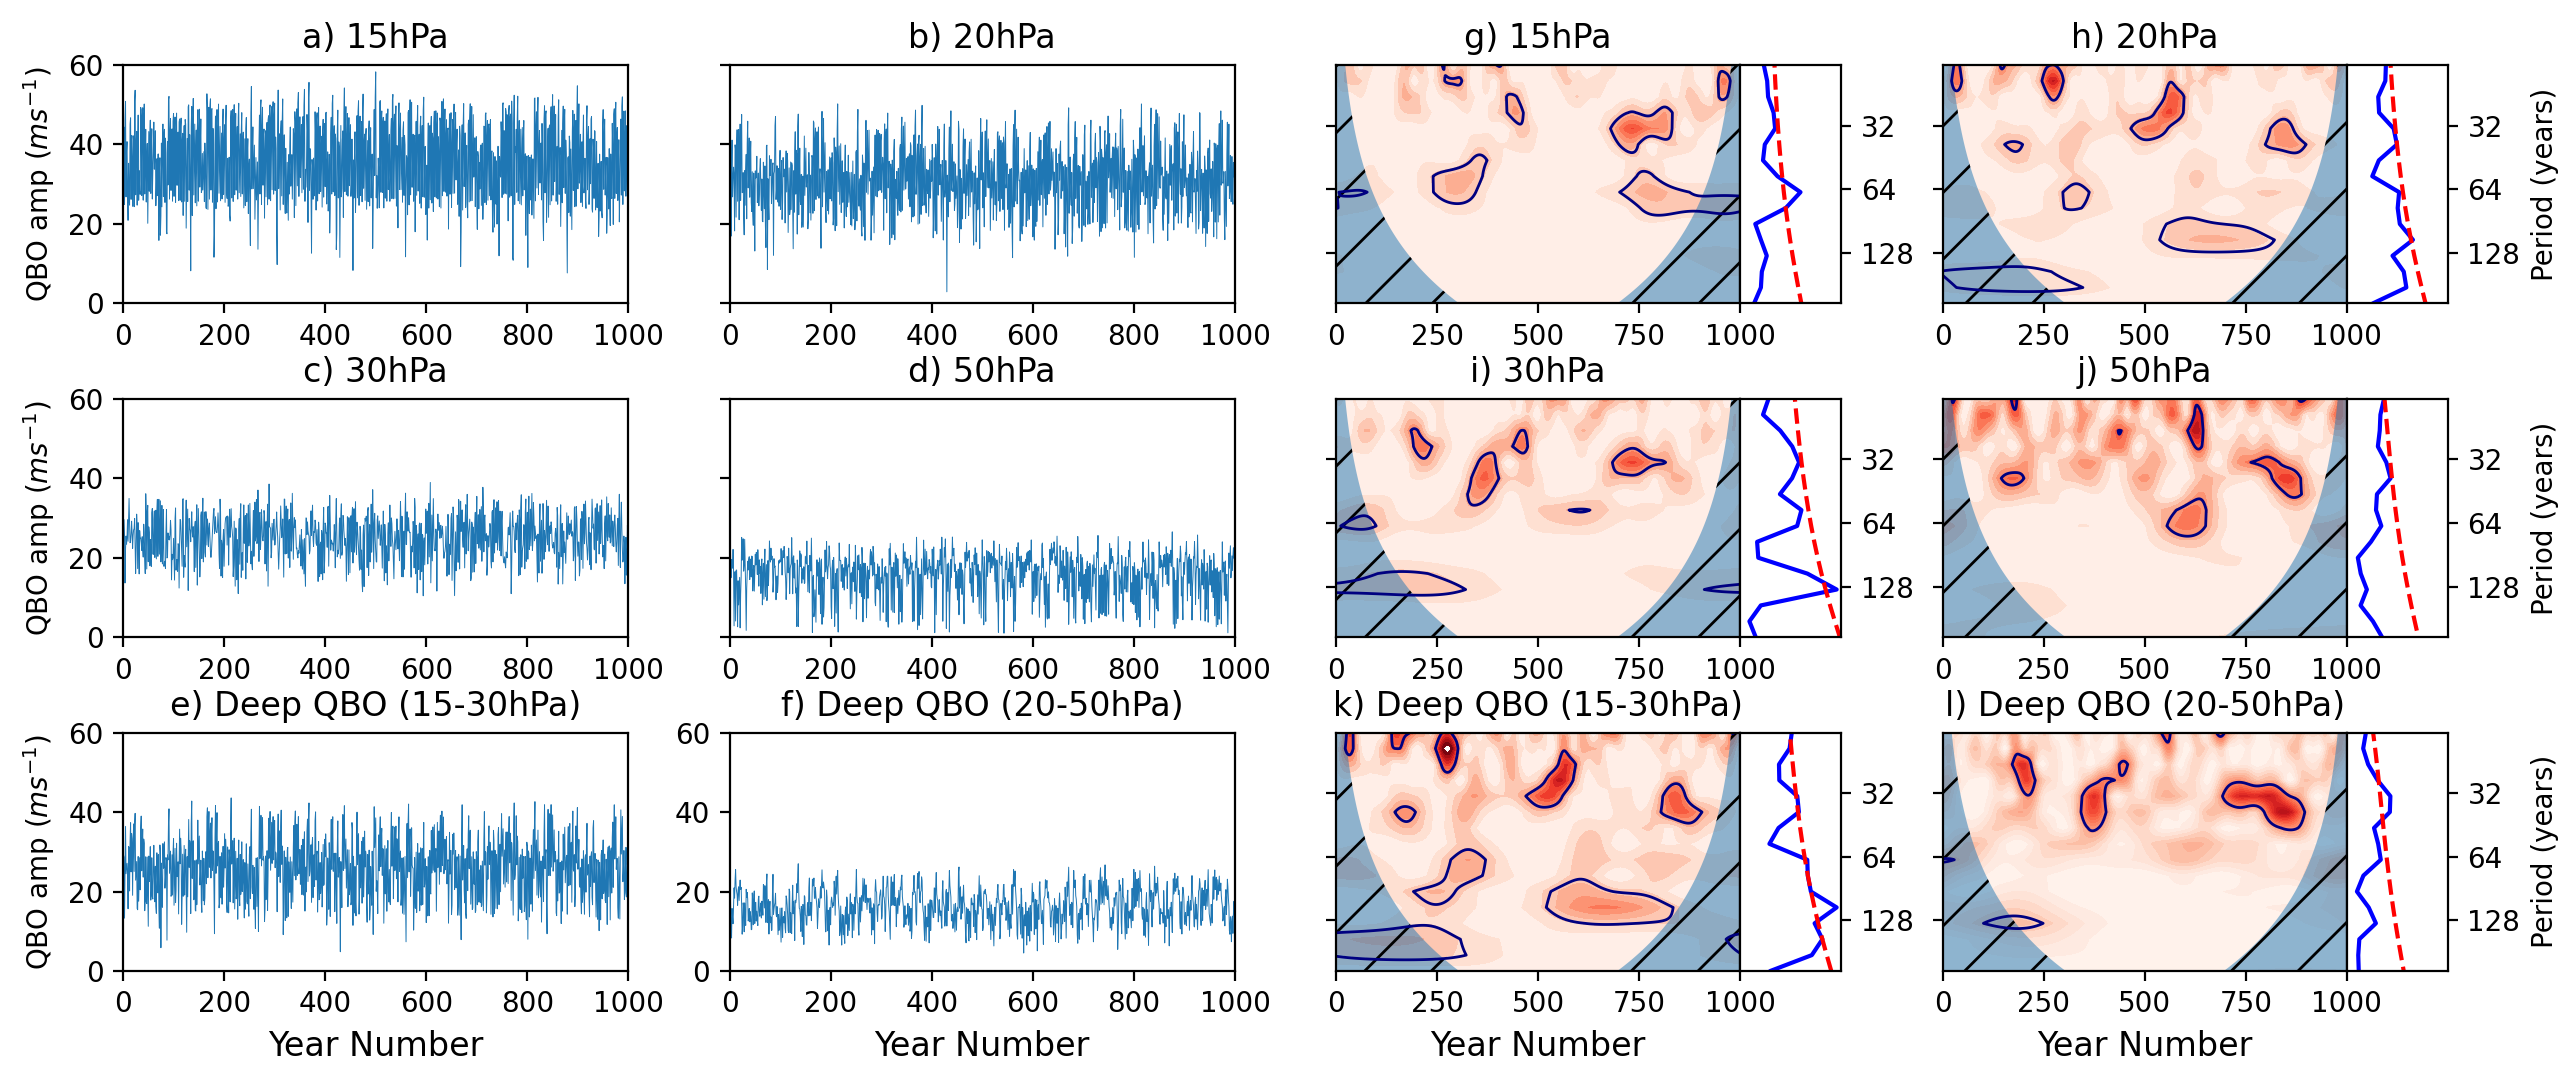
\includegraphics[width = \linewidth]{Figures/Figures-origins/QBO_levels_amp.png}
\caption{\textbf{(a-e)}: Hilbert amplitude of Sep-Nov mean ZMZW averaged between 5$^\circ$\,S--5$^\circ$\,N latitude on different pressure levels (a-e) and the deep metric averaged between 15--30\,hPa (f). \textbf{(g-l)}: Wavelet power spectra for each time series shown in (a-c). Shading represents wavelet power with a colour scale the same as that seen in figure 6 and yellow contours indicate regions of significant power (>95\% confidence interval) compared to a background AR1 process.}
\label{QBO_levs_amp}
\end{figure}
\end{center}

%---------------------------------------------------------------

Wavelet analysis of the 5-year smoothed deep (15-30\,hPa) QBO amplitude modulation index (figure 12a) enhances the clarity of the long-term periodicity, showing statistically significant power at around 90 years in the interval between year numbers 500-800. The cross power between $SSW_5yr$ and this QBO amplitude modulation index (figure \ref{fig:QBO_SSW_subfig}) coincides extremely well with the signals observed in $SSW_5yr$ at around 90 years. There are also coincident features at other timescales, although the feature between years 450-550 at periods of 60 years is less well captured. The phase-relationship arrows in the main region of long-term variability (periods around 90 years in the interval 450-800 years) point broadly to the left ($\pi$ phase shift), indicating that the signals are approximately anti-phased (the slight downward pointing of the arrows suggests a small deviation from this lag-zero relationship and is discussed below). The anti-phase relationship is consistent with the HT relationship in which a westerly (positive) QBO anomaly corresponds to a reduction in the frequency of SSWs.

%---------------------------------------------------------------

\begin{center}
\begin{figure}[h!]
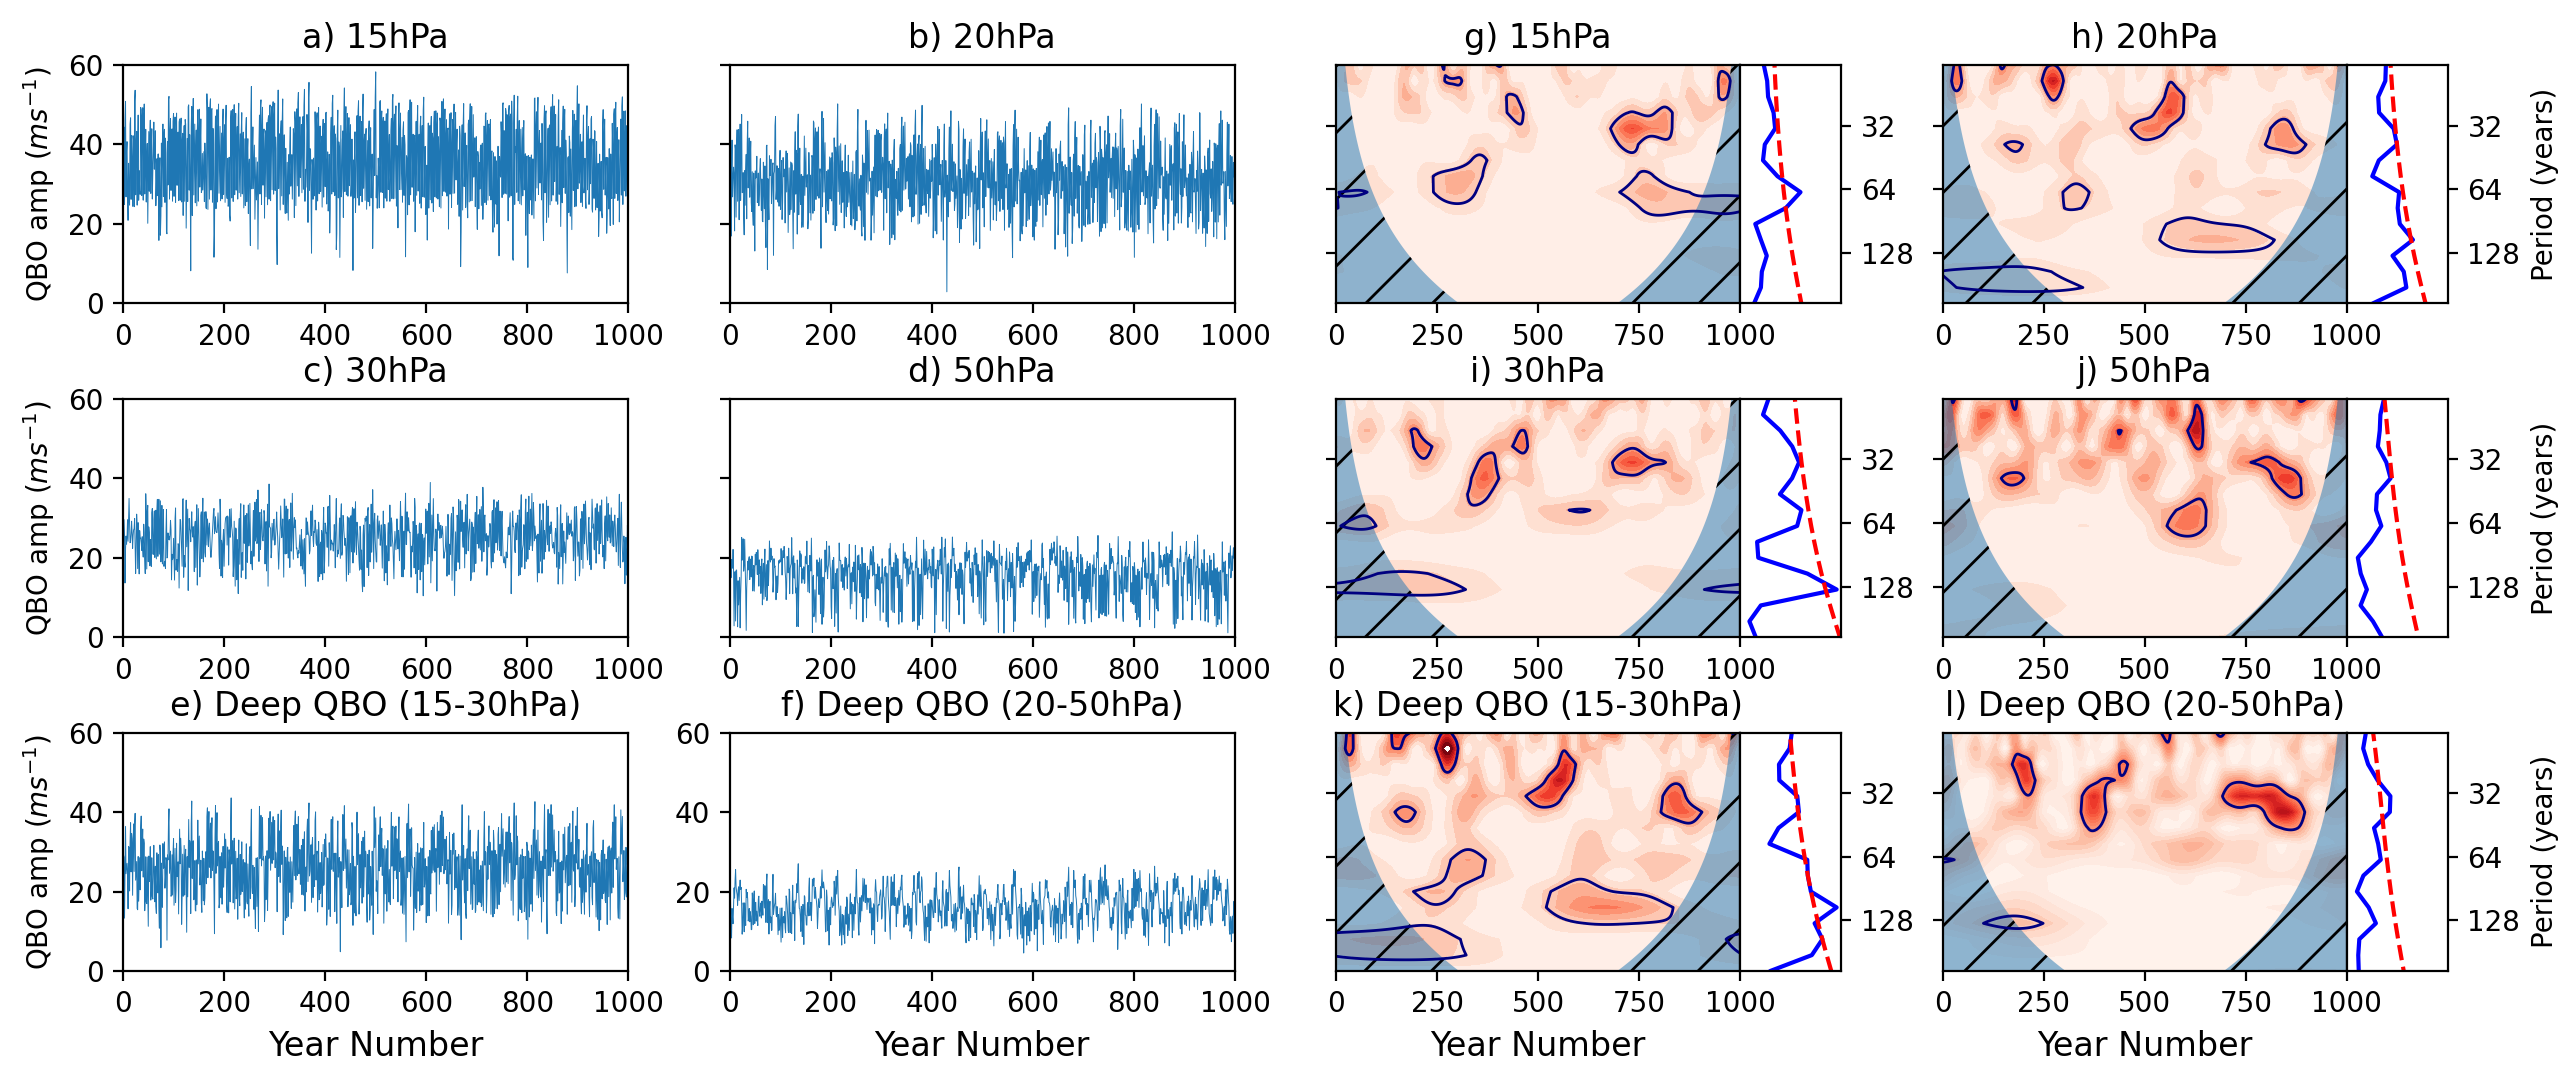
\includegraphics[width = \textwidth]{Figures/Figures-origins/QBO_levels_amp.png}
\caption{As figure 8 for the Sep-Nov deep QBO (15--30\,hPa) amplitude index smoothed with a 5 year window. \textbf{a}: QBO amplitude time series and associated wavelet power spectrum,\textbf{b}: Cross power spectrum between deep QBO amplitude and $SSW_5yr$.}
\label{fig:QBO_SSW_subfig}
\end{figure}
\end{center}

%---------------------------------------------------------------


In our earlier discussion we linked long-term variability in SSW frequency to the existence of extended hiatus periods, during which the vortex is relatively undisturbed with no SSW events (figure 2). The cross-spectrum analysis with deep QBO amplitude modulation suggests a possible physical interpretation involving the Holton-Tan relationship varying on longer timescales, in which a series of consecutive years that exhibit a large amplitude, deep westerly QBO in early winter leads to a series of winters with reduced SSW frequency i.e. a hiatus period. Correspondingly a series of large-amplitude deep easterly QBO years would lead to a series of consecutive-event years.

We verify the results of the wavelet analyses described above by repeating the multi-linear regression (table 1) but using the 5-year smoothed QBO, ENSO and AL indices to measure their  relative contributions to the 5-year smoothed  $SSW_5yr$ time-series. The resulting regression coefficients for the deep QBO amplitude and AL remain significant at the 95\% level, although the AL's contribution remains small and close to the significance boundary. The coefficient for ENSO3.4 is not significant, suggesting that the connection between this ENSO index and the vortex variability is dominated by timescales less than 5 years. If we further isolate multi-decadal signals by fourier filtering each timeseries, so that only periodicities longer than 60 years are retained, the ENSO3.4 coefficient is near 0 while the deep QBO amplitude signal is near -0.2. This is consistent with our wavelet analysis which suggest a dominant role for QBO amplitude variations on these long timescales. The AL coefficient remains significant but smaller than that of the QBO (and outside error ranges). For completeness, we repeated the regression analysis using a 5-year smoothed PDO index instead of the AL but there was no significant change in the coefficients (not shown). This is consistent with the fact that the AL and PDO indices exhibit similar spectra and there is a high correlation between them (-0.45 unfiltered and -0.68 filtered), as also found by \cite{mantuaPacific1997} and \cite{rodionovSpatial2005}. 

\begin{table}
\centering
\begin{tabular}{|p{3cm}||p{3cm}|p{3cm}|}
 \hline
 \multicolumn{3}{|c|}{SSW$_{5yr}$ regression}\\
 \hline
 Regression Variable& Coefficient& p value\\
 \hline
 ENSO3.4  & -0.0127$\pm$0.032& 0.688\\
 AL  &   -0.072$\pm$0.021  & 0.046\\
 deep QBO amp &-0.124$\pm$0.031&0.0001\\
 \hline
\end{tabular}
\begin{center}
\caption{Summary of results from multi-linear regression analysis of SSW$_{5yr}$.} 
\end{center}
\end{table}

\begin{table}
\centering
\begin{tabular}{|p{3cm}||p{3cm}|p{3cm}|}
 \hline
 \multicolumn{3}{|c|}{Filtered (>60 year periods) SSW$_{5yr}$ regression}\\
 \hline
 Regression Variable& Coefficient& p value\\
 \hline
 ENSO3.4  &   $\sim$0$\pm$0.01  & $\sim$1\\
 AL & -0.0794$\pm$0.03& 0.042\\
 deep QBO amp &-0.199$\pm$0.01&0.00003\\
 \hline
\end{tabular}
\begin{center}
\caption{Summary of results from multi-linear regression analysis of a fourier filtered  version of SSW$_{5yr}$ retaining power corresponding to periods greater than 60 years.}  
\end{center}
\end{table}
